\documentclass[11pt]{article}
\usepackage[a4paper, total={6in, 8.5in}]{geometry}
\usepackage[english]{babel}
\usepackage{graphicx}
\usepackage{hyperref}
\usepackage[onehalfspacing]{setspace}
\usepackage{float}
\usepackage{titlepic}
\usepackage{listings}
% \usepackage{xcolor}
\usepackage{amsmath}
\usepackage{amsfonts}
\usepackage{scrlayer-scrpage}
\usepackage{csquotes}
\usepackage{blkarray}
\usepackage{mwe}
\usepackage{algorithm}
\usepackage{algorithmic}
\usepackage{esvect}
\usepackage{physics}
\usepackage[table,xcdraw]{xcolor}


\usepackage[style=authoryear, backend=biber]{biblatex}
\usepackage{amssymb}
\addbibresource{references.bib}
\cfoot*{\pagemark}

\DeclareMathOperator*{\argmax}{arg\,max}
\DeclareMathOperator*{\argmin}{arg\,min}
\newcommand{\E}{\mathrm{E}}
\newcommand{\Var}{\mathrm{Var}}
\newcommand{\Cov}{\mathrm{Cov}}



\begin{document}
    \title{Autonomous Systems - Perception, Potential Fields}
    \date{06/2021}
    \author{Rupp Matthias}
    \maketitle
    \thispagestyle{empty}
    \vspace{2 cm}
    \begin{figure}[H]
        \centering
        
\includegraphics[width = 6cm]{Logo-A3}\label{fig:logo}
    \end{figure}
    \pagebreak

    \ohead{Rupp Matthias}
    \tableofcontents
    \thispagestyle{empty}
    \clearpage

    \definecolor{codegreen}{rgb}{0,0.6,0}
    \definecolor{codegray}{rgb}{0.5,0.5,0.5}
    \definecolor{codepurple}{rgb}{0.58,0,0.82}
    \definecolor{backcolour}{rgb}{0.95,0.95,0.92}

    \lstdefinestyle{mystyle}{
        backgroundcolor=\color{backcolour},
        commentstyle=\color{codegreen},
        keywordstyle=\color{magenta},
        numberstyle=\tiny\color{codegray},
        stringstyle=\color{codepurple},
        basicstyle=\ttfamily\footnotesize,
        breakatwhitespace=false,
        breaklines=true,
        captionpos=b,
        keepspaces=true,
        numbers=left,
        numbersep=5pt,
        showspaces=false,
        showstringspaces=false,
        showtabs=false,
        tabsize=2
    }
    \lstset{style=mystyle}

    \section{Graphics}\label{sec:graphics}
    \begin{figure}[H]
        \centering
        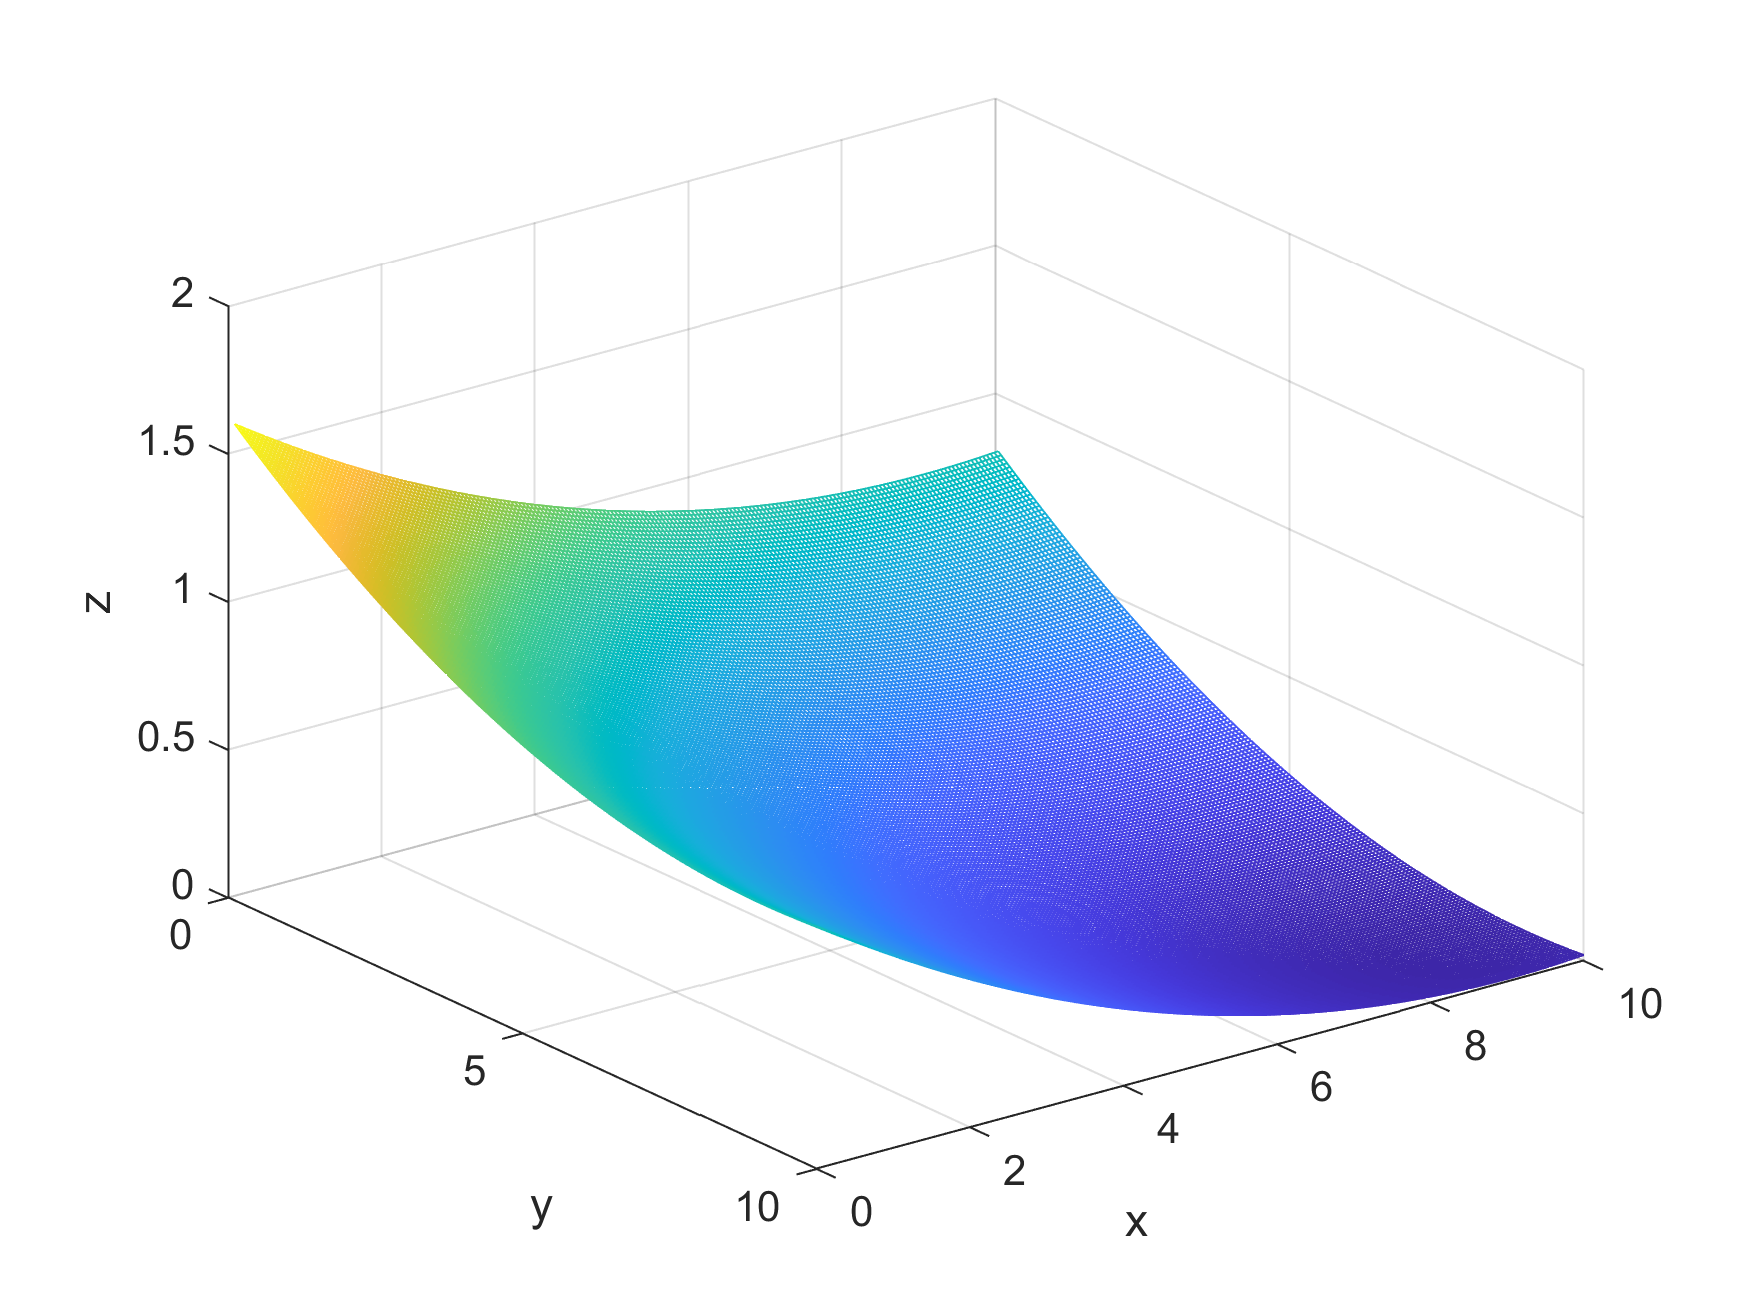
\includegraphics[width=1.0\textwidth]{../test/images/u_att}
        \caption{Attracting field}
        \label{fig:attfield}
    \end{figure}

    \begin{figure}[H]
        \centering
        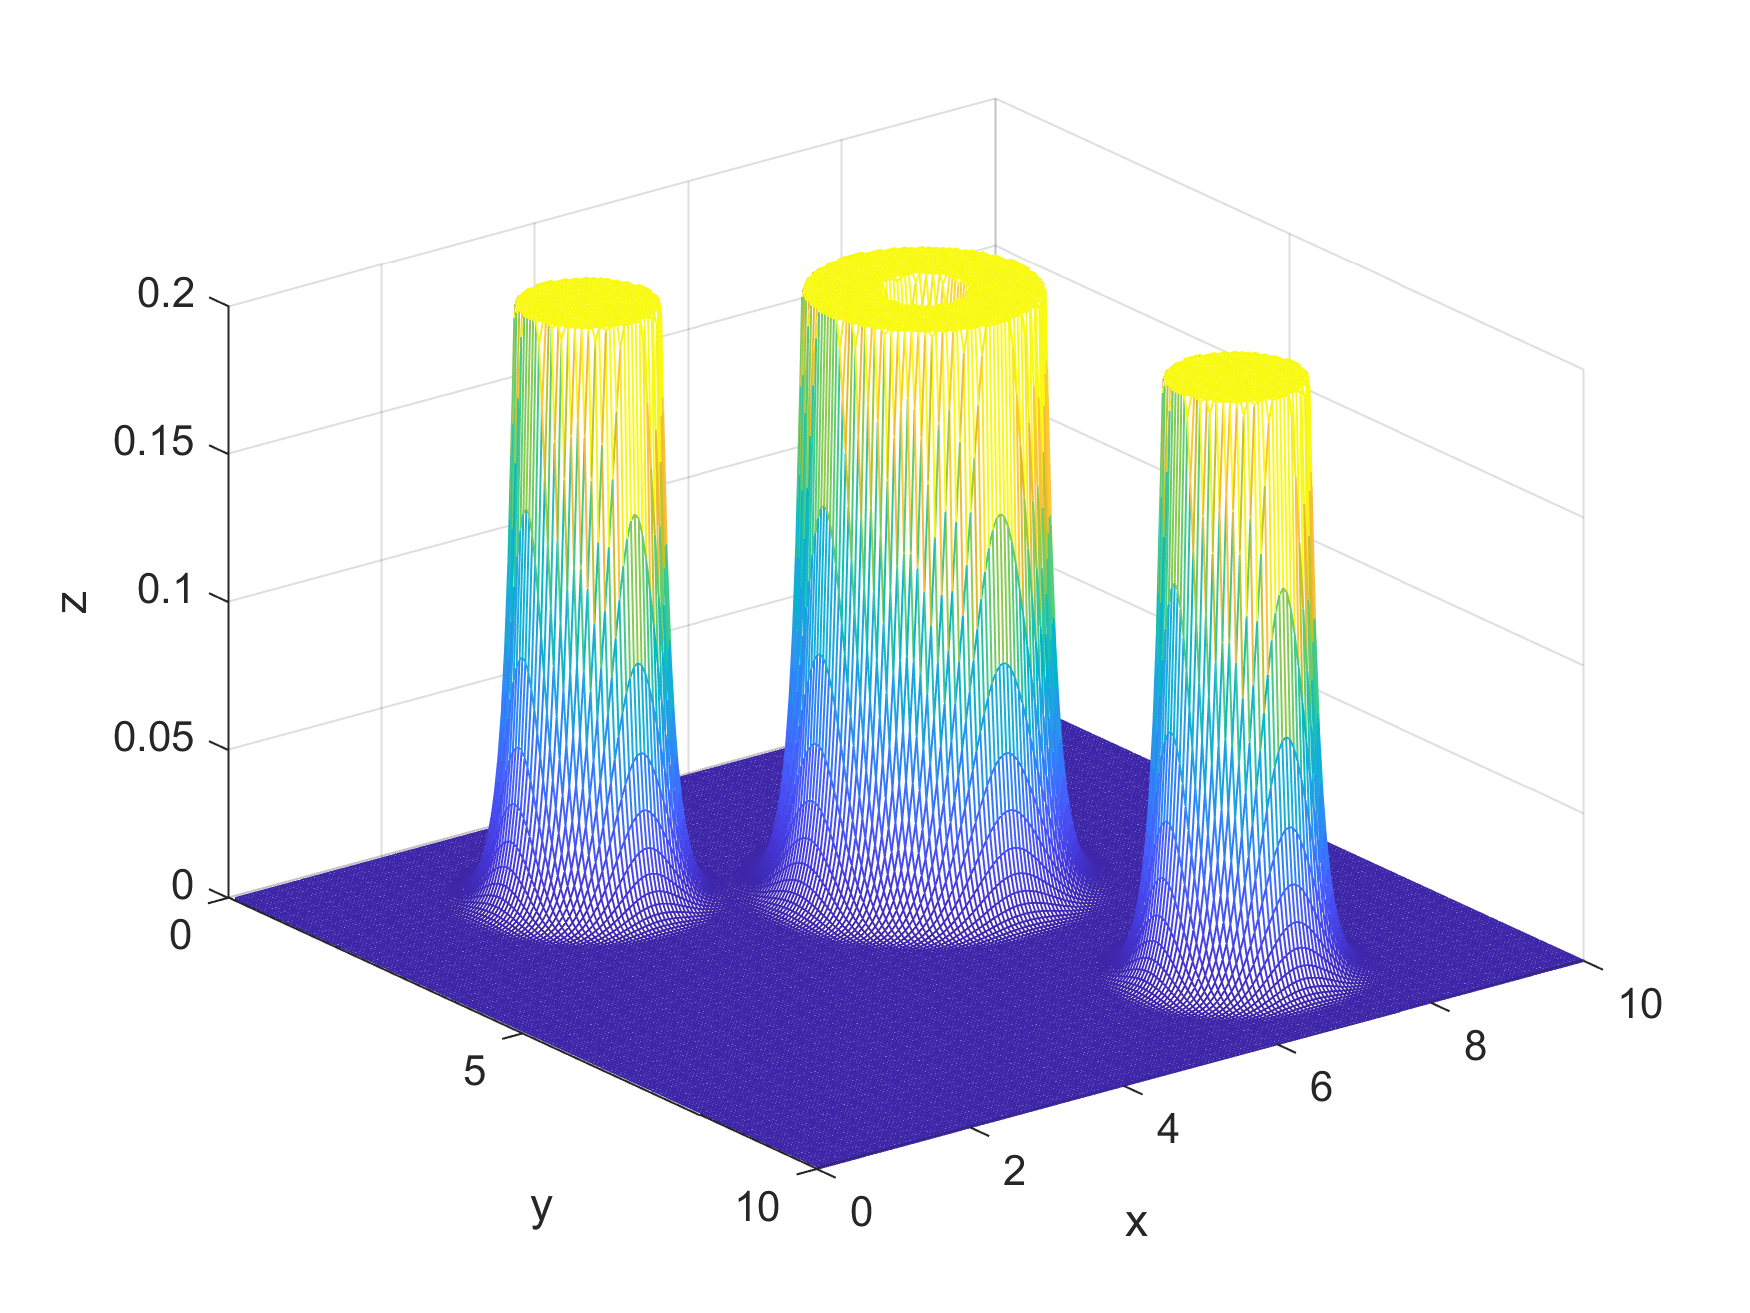
\includegraphics[width=1.0\textwidth]{../test/images/u_rep}
        \caption{Repelling field}
        \label{fig:repfield}
    \end{figure}

    \begin{figure}[H]
        \centering
        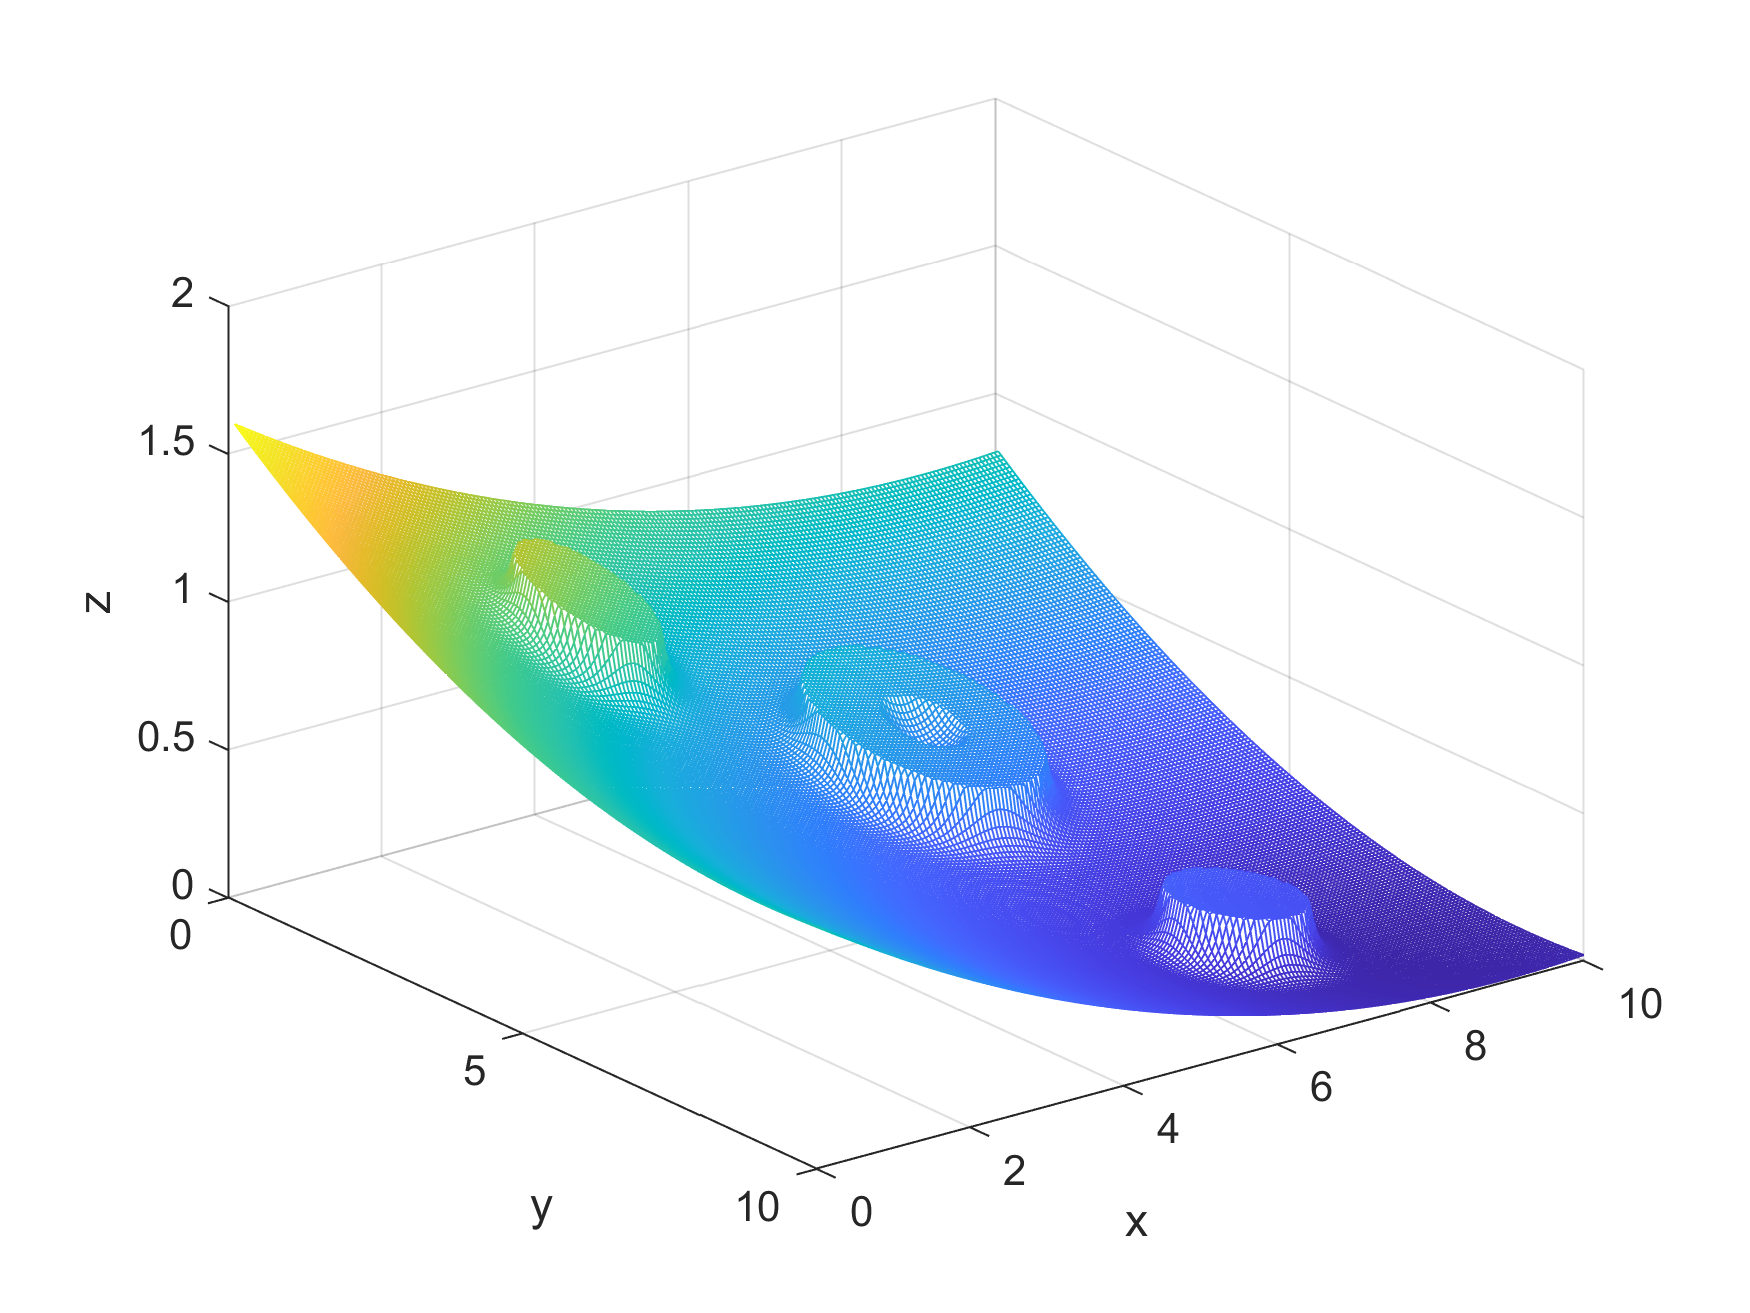
\includegraphics[width=1.0\textwidth]{../test/images/u_combi}
        \caption{Total potential field}
        \label{fig:potfield}
    \end{figure}

    \begin{figure}[H]
        \centering
        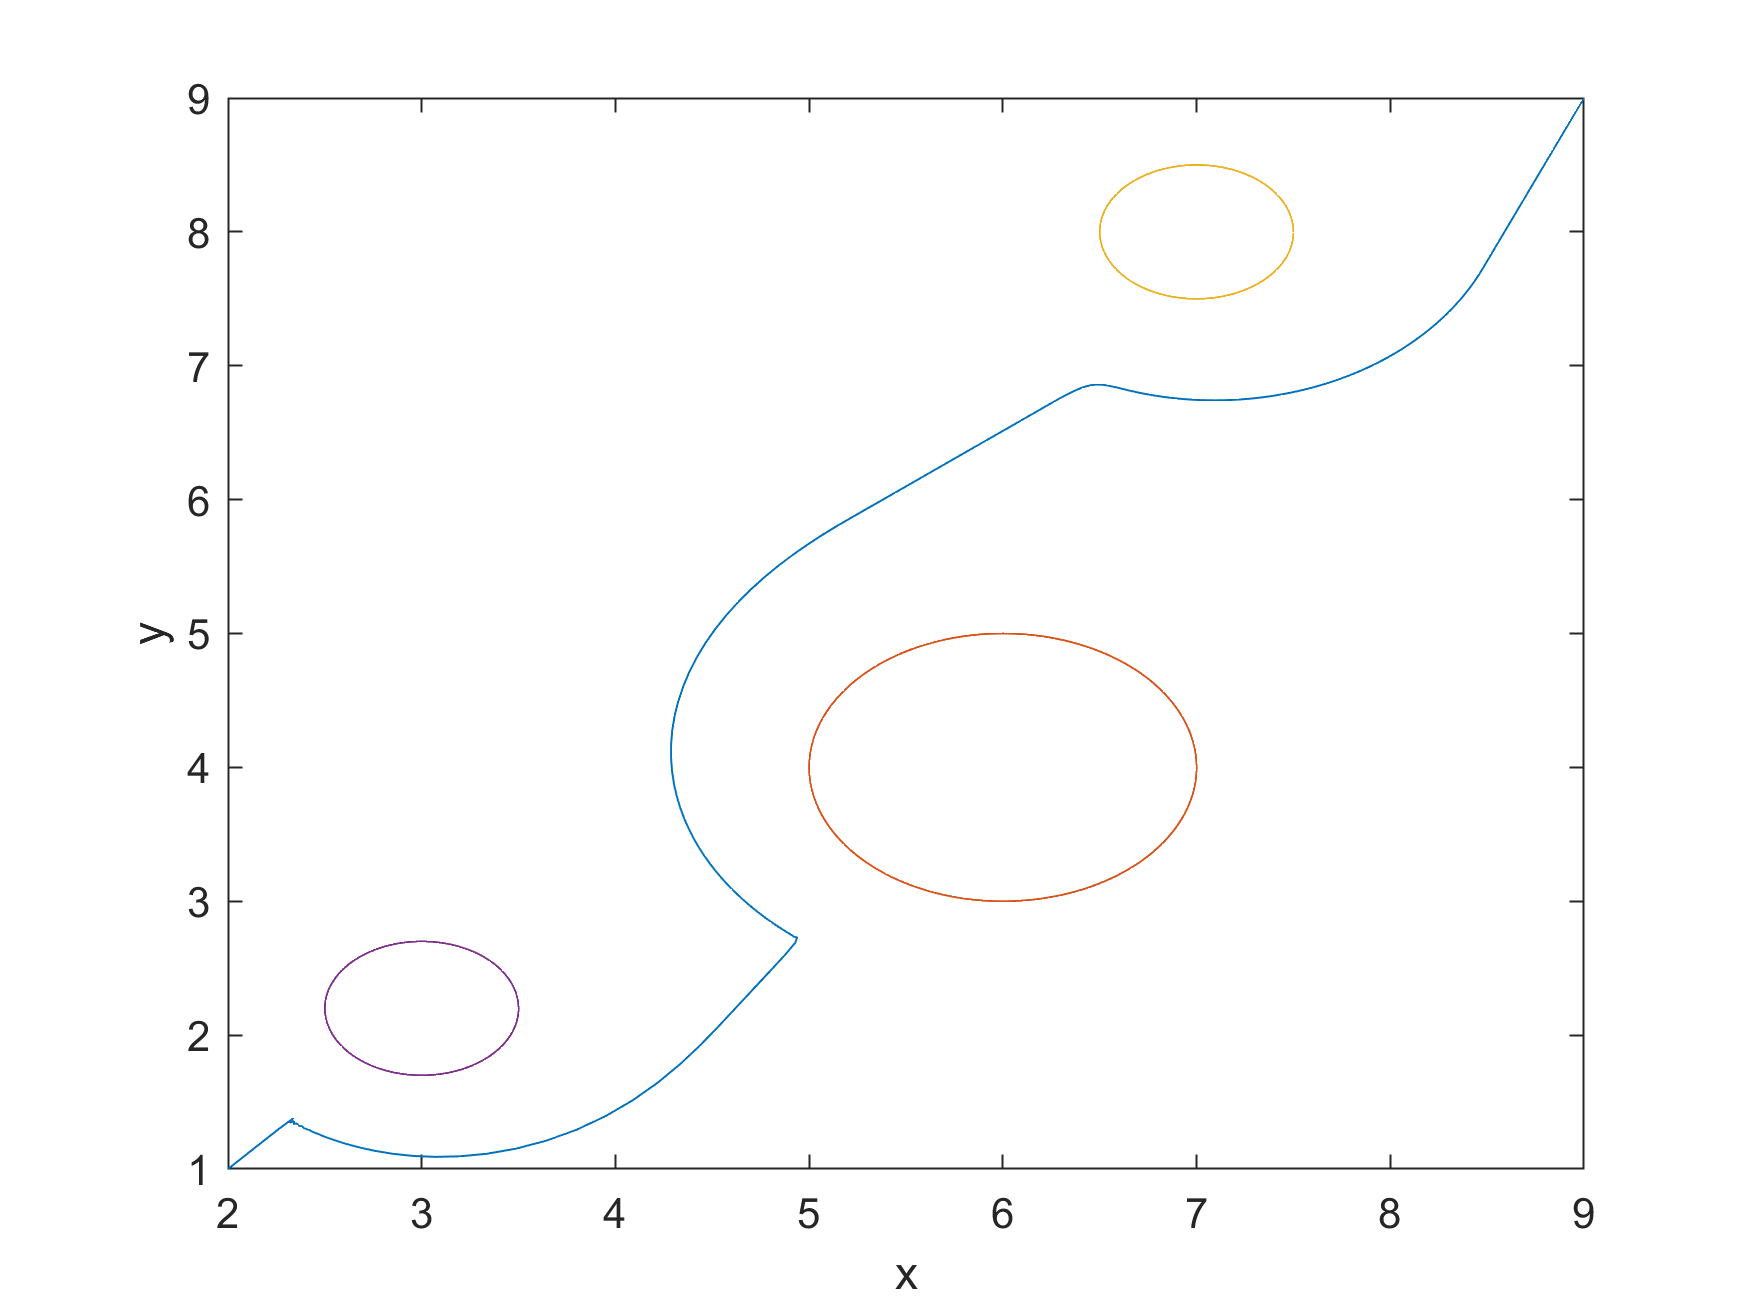
\includegraphics[width=1.0\textwidth]{../test/images/robot_path}
        \caption{Robot path through potential field}
        \label{fig:robpath}
    \end{figure}

    \clearpage
    \phantomsection
    \addcontentsline{toc}{section}{References}
    \printbibliography

    \clearpage
    \phantomsection
    \addcontentsline{toc}{section}{List Of Figures}
    \listoffigures


\end{document}